\documentclass{article} % For LaTeX2e
\usepackage{nips15submit_e,times}
\usepackage{hyperref}
\usepackage{url}
\usepackage{graphicx}
\graphicspath{ {/Users/Tyler/LOVEFest/Figures/pdf/} }
%\documentstyle[nips14submit_09,times,art10]{article} % For LaTeX 2.09
\usepackage{amsfonts}
\usepackage{amsmath}


\title{Randomer Forests}


\author{
Tyler M. Tomita\thanks{ Use footnote for providing further information
about author (webpage, alternative address)---\emph{not} for acknowledging
funding agencies.} \\
Department of Biomedical Engineering\\
Johns Hopkins University\\
Baltimore, MD \\
\texttt{ttomita@jhu.edu} \\
\And
Joshua T. Vogelstein \\
Department of Biomedical Engineering \\
Johns Hopkins University \\
\texttt{email} \\
\AND
Coauthor \\
Affiliation \\
Address \\
\texttt{email} \\
\And
Coauthor \\
Affiliation \\
Address \\
\texttt{email} \\
\And
Coauthor \\
Affiliation \\
Address \\
\texttt{email} \\
(if needed)\\
}

% The \author macro works with any number of authors. There are two commands
% used to separate the names and addresses of multiple authors: \And and \AND.
%
% Using \And between authors leaves it to \LaTeX{} to determine where to break
% the lines. Using \AND forces a linebreak at that point. So, if \LaTeX{}
% puts 3 of 4 authors names on the first line, and the last on the second
% line, try using \AND instead of \And before the third author name.

\newcommand{\fix}{\marginpar{FIX}}
\newcommand{\new}{\marginpar{NEW}}

%\nipsfinalcopy % Uncomment for camera-ready version

\begin{document}

\maketitle

\begin{abstract}
Insert abstract
\end{abstract}

\section{Introduction}
Insert introduction

\section{Randomer Forests}
A random forest is an ensemble of randomized decision trees, where each decision tree consists of internal (split) and terminal (leaf) nodes. At each internal node, a random subset of the ambient (coordinate) dimensions is sampled and subsequent optimization of a split function selects the single best dimension and split point contained in this subset. Therefore, each tree within a random forest can be viewed as a hierarchical series of axis-aligned decision boundaries. Here, we introduce a new method for constructing randomized decision trees, where instead of random subsampling the dimensions, we randomly project to a lower dimensional subspace. By randomly projecting, decision boundaries are not restricted to alignment with the coordinate axes. Specifically, let $X \in \mathbb{R}^{nxp}$ be a set of n points in p dimensional Euclidean space and $R \in \mathbb{R}^{pxk}$ be a randomly chosen projection matrix. At each internal node, we compute the projection $X_k = XR$ and select the optimal split dimension and split point in this randomly chosen k-dimensional subspace.

There exists various choices for the random projection matrix $R$. In this work, we look at two, which we will denote as dense (d) and sparse (s). We define dense random matrices such that each element $r_{ij}$  of $R$ is distributed as \begin{align*}
&P(r_{ij} = -1) = 1/6 \\
&P(r_{ij} = 0) = 2/3 \\
&P(r_{ij} = +1) = 1/6
\end{align*}
To sample a sparse matrix, first, the indices of k nonzero elements in the matrix is sampled uniformly at random. Each nonzero element is then randomly assigned -1 or +1 with equal probability. Columns containing all zeros are removed. This results in a matrix with many columns having one nonzero element and a few columns having more than one nonzero element.

In addition to random projections, for classification problems involving $c$ classes we can compute a set of $c-1$ differences in class-conditional means $\{\boldsymbol{\delta_{ij}} = \boldsymbol{\mu_j} - \boldsymbol{\mu_i}: \forall i \in [1,...,c-1], j \in [2,...,c], j>i\}$ and sample each of them as a projection with probability $k/p$. Such supervised projections work especially well when all classes are normally distributed with diagonal covariance matrices, and are often useful even when these conditions are not met. We denote RerFs utilizing these projections as RerF($\delta$)

When taking linear combinations of ambient dimensions, it is important that the dimensions be scaled similarly. Therefore we also formulate a variant of RerF in which input data is passed to marginal ranks prior to training. Doing so not only scales the dimensions appropriately, but also can improve performance when outliers are present. This robust variant of randomer forest will be denoted as RerF(r).

\section{Experimental Evaluation}

\subsection{Simulated Data}
We constructed three synthetic datasets (Trunk, parity, and multimodal) to compare classification performance (Fig 1) and training time (Fig 2) of RerF(d), RerF(s), RerF(s+$\delta$), and RerF(s+$\delta$+r) with that of random forest. Trunk is a well-known binary classification \cite{} in which each class is distributed as a p-dimensional multivariate gaussian with identity covariance matrices. The means of the two classes are $\mu_1 = (1,\frac{1}{\sqrt{2}},\frac{1}{\sqrt{3}},...,\frac{1}{\sqrt{p}})$ and $\mu_2 = (-1,-\frac{1}{\sqrt{2}},-\frac{1}{\sqrt{3}},...,-\frac{1}{\sqrt{p}})$. Parity is a binary classification problem in which each of the two classes is distributed as a mixture of $2^{p-1}$ multivariate gaussians with covariance matrices $\boldsymbol{\Sigma} = \frac{1}{32}\boldsymbol{I}$. The means of class one are the subset of $[0,1]^p$ for which the number of zeros in a mean is even. The means of class two are the subset of $[0,1]^p$ for which the number of zeros in a mean is odd. Multimodal is a four-class classification problem. Each of the four classes is distributed as an equal mixture of two multivariate gaussians. The means are randomly sampled from a p-dimensional multivariate gaussian and the covariance matrices are sampled from an inverse Wishart distribution with $10p$ degrees of freedom and  a mean covariance matrix equal to the identity matrix. The bottom panels of Figure 1 depict scatter plots of the data for $p=2$. The top panels depict average misclassification rate over ten trials estimated using the out of bag error. For the trunk and multimodal simulations, 100 points were sampled and p varied from two to 1000 dimensions. For the parity simulation, 100 points were sampled and p varied from two to ten. The appropriate number of trees trained for RF and all variants of RerF for trunk, parity, and multimodal were empirically determined to be 1500, 1000, and 500 respectively (Fig S1). Bayes error is also included for reference. In binary classification problems in which each class consists of a single multivariate gaussian with equal covariance matrices, such as theTrunk simulation, Bayes error can be computed analytically (Bickel and Levina 2004). In the Parity and Multimodal simulations, Bayes error was estimated by averaging the misclassification rate of the Bayes optimal classifier on 1000 points over ten trials.

Panel A of Figure 1 shows that RerF(s+$\delta$) and RerF(s+$\delta$+r) outperform RF across all numbers of dimensions. This can be attributed to projection onto the difference in means. All variants outperform RF up to approximately 250 dimensions. Above this, misclassification rate of RerF(s) is comparable to RF and misclassification rate of RerF(d) is larger. The degradation in performance of RerF(d) above 250 dimensions is due to projections containing a large number of noisy dimensions. In Panel B, we observe that all variants of RerF outperform RF for all numbers of dimensions. This can be understood by observing that for p dimensions, all splits in RF up to a tree depth of $p - 1$ will result in daughter nodes having chance posterior probabilities of being in either class. Therefore, any splits up to this depth that are not aligned with the coordinate axes can only be better. Multimodal???

In Figure 2, we observe a slight increase training time of all RerF variants compared to RF. Despite this increase, training time for all classifiers scales similarly with the number of dimensions. The apparent increase in training time for the RerF variants is largely due to sampling of the random projection matrices. 


\subsection{Effects of Transformations and Outliers on Classifier Performance}

RF does especially well in classification problems in which the optimal decision boundaries are aligned or close to aligned with the coordinate axes. Rotations in such situations can lead to a decrease in classification performance. Naturally, we wanted to examine the effects of various transformations on classification performance of RerF. These effects were examined using the Trunk and parity simulations as previously described. The transformations we applied were random rotations, scaling, and general affine transformations. Uniformly random rotation matrices were generated by first performing SVD on a p-dimensional matrix in which each element is sampled from a multivariate standard normal distribution. The rotation matrix was taken as the right singular vectors of this SVD. If the determinant of this matrix was equal to $-1$, the first two columns were permuted to render the determinant equal to $+1$. Random scaling was performed by applying to each dimension a scaling factor sampled from a uniform distribution on the interval [0,10]. Affine transformations were performed by applying a combination of rotations and scalings as just described. Additionally, we examined the effects of introducing outliers. Outliers were introduced to Trunk and parity simulations by sampling points from the distributions as previously described but instead using covariance matrices scaled by a factor of four. Empirically, an addition of 20 points from these outlier models to the original 100 points was found to produce a noticeable but not overwhelming effect on classifier performance. The classifiers evaluated were RF, RF(s), RF(s+$\delta$). Additionally, Fisherfaces was evaluated as a reference. The misclassification rate for Fisherfaces was estimated using leave-one-out cross validation. 

The top panels of Figure 4 illustrate the effects of the transformations and outliers on the Trunk simulation. The bottom panels show these effects on the parity simulation. In the Trunk simulation, rotation results in noticeable degradation in classification performance of RF when the number of dimensions is greater than approximately 100. On the other hand, both RerF(s+$\delta$) and RerF(s+$\delta$+r) are unaffected by rotations. RerF(s+$\delta$) exhibits an increase in misclassification rate when scaling is applied. This is expected because ambient dimensions with a relatively large scale will dominate the variance of new dimensions constructed from a linear combination of the ambient ones. For this same reason, Fisherfaces is also affected by scaling. Since RerF(s+$\delta$+r) maps all dimensions to the same scale, it is invariant to scaling and is also the only classifier to exhibit invariance to affine transformations. We also observe that all classifiers are only slightly affected by the addition of outliers to the Trunk simulation. As shown in panel E, rotations in the Parity simulation actually improve classification performance of RF. As mentioned previously, all splits in RF up to a tree depth of $p - 1$ in the untransformed parity simulation result in chance probabilities of being in either class in the daughter nodes. Therefore, rotating can only improve performance. As in the Trunk simulation, performance of RerF(s) is hurt when scaling is applied in the parity simulation.

\subsection{Real Data}

In addition to the simulations, RF, RerF(d), RerF(s), RerF(s+$\delta$), and RerF(s+$\delta$+r) were evaluated on 121 datasets as described in \cite{}. Classifiers were trained on the entire training sets provided. For each data set, misclassification rates were again estimated by out of bag error, and training time was measured as wall clock time. Misclassification rates and training times were averaged over all 121 datasets (Fig 4).

\section{Discussion}

Insert discussion

\begin{figure}[h]
\begin{center}
%\framebox[4.0in]{$\;$}
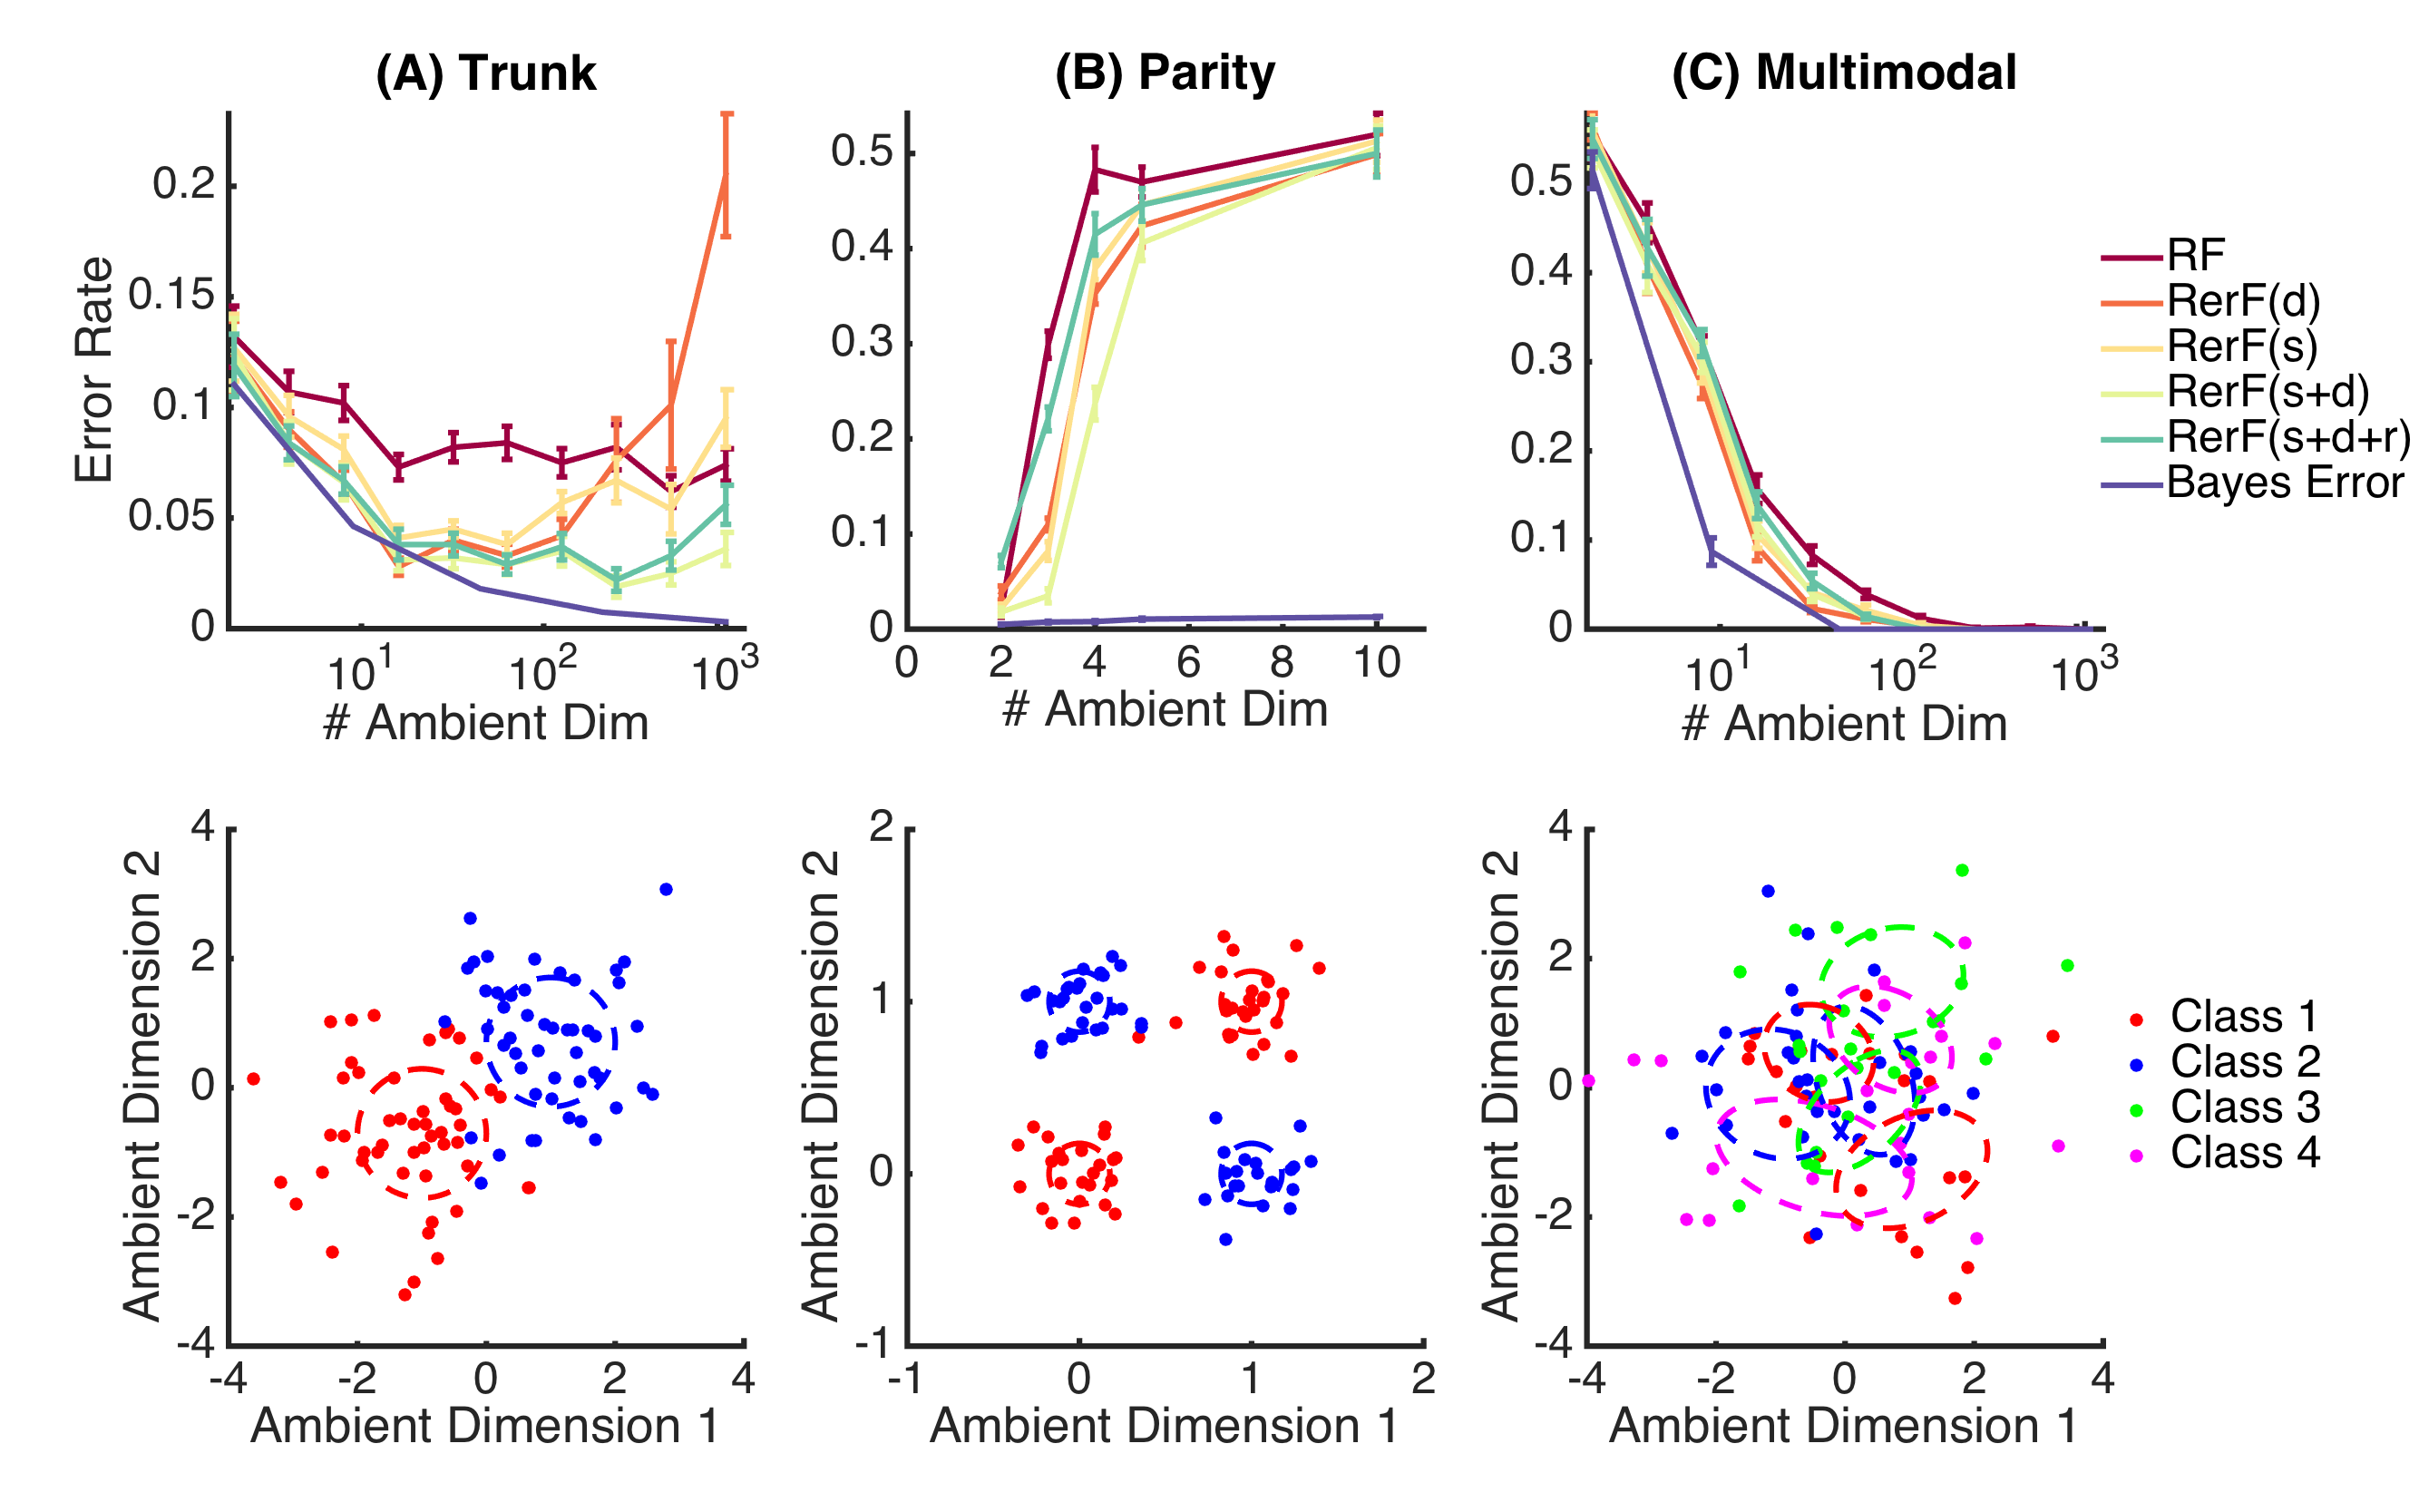
\includegraphics[trim=0in 0.4in 0in 0.4in, clip=true, width=\linewidth]{Fig1_Lhat}
\end{center}
\caption{Classification performance comparing Random Forest (RF) to several variants of Randomer Forest (RerF), and Bayes optimal performance, on three distinct simulation settings: (A) Trunk, (B) Parity, and (C) Multimodal (see Methods for details).  For all settings, the top panel depicts misclassification rate vs. the number of ambient (coordinate) dimensions, and the bottom panel shows a 2D scatter plot of the first 2 coordinates (dashed circles denote the standard deviation level set).  Note that in all settings, for all number of dimensions, RerF outperforms RF, even Trunk and Parity, which were designed specifically for RF because the discriminant boundary naturally lies along the coordinate basis.}
\end{figure}

\begin{figure}[h]
\begin{center}
%\framebox[4.0in]{$\;$}
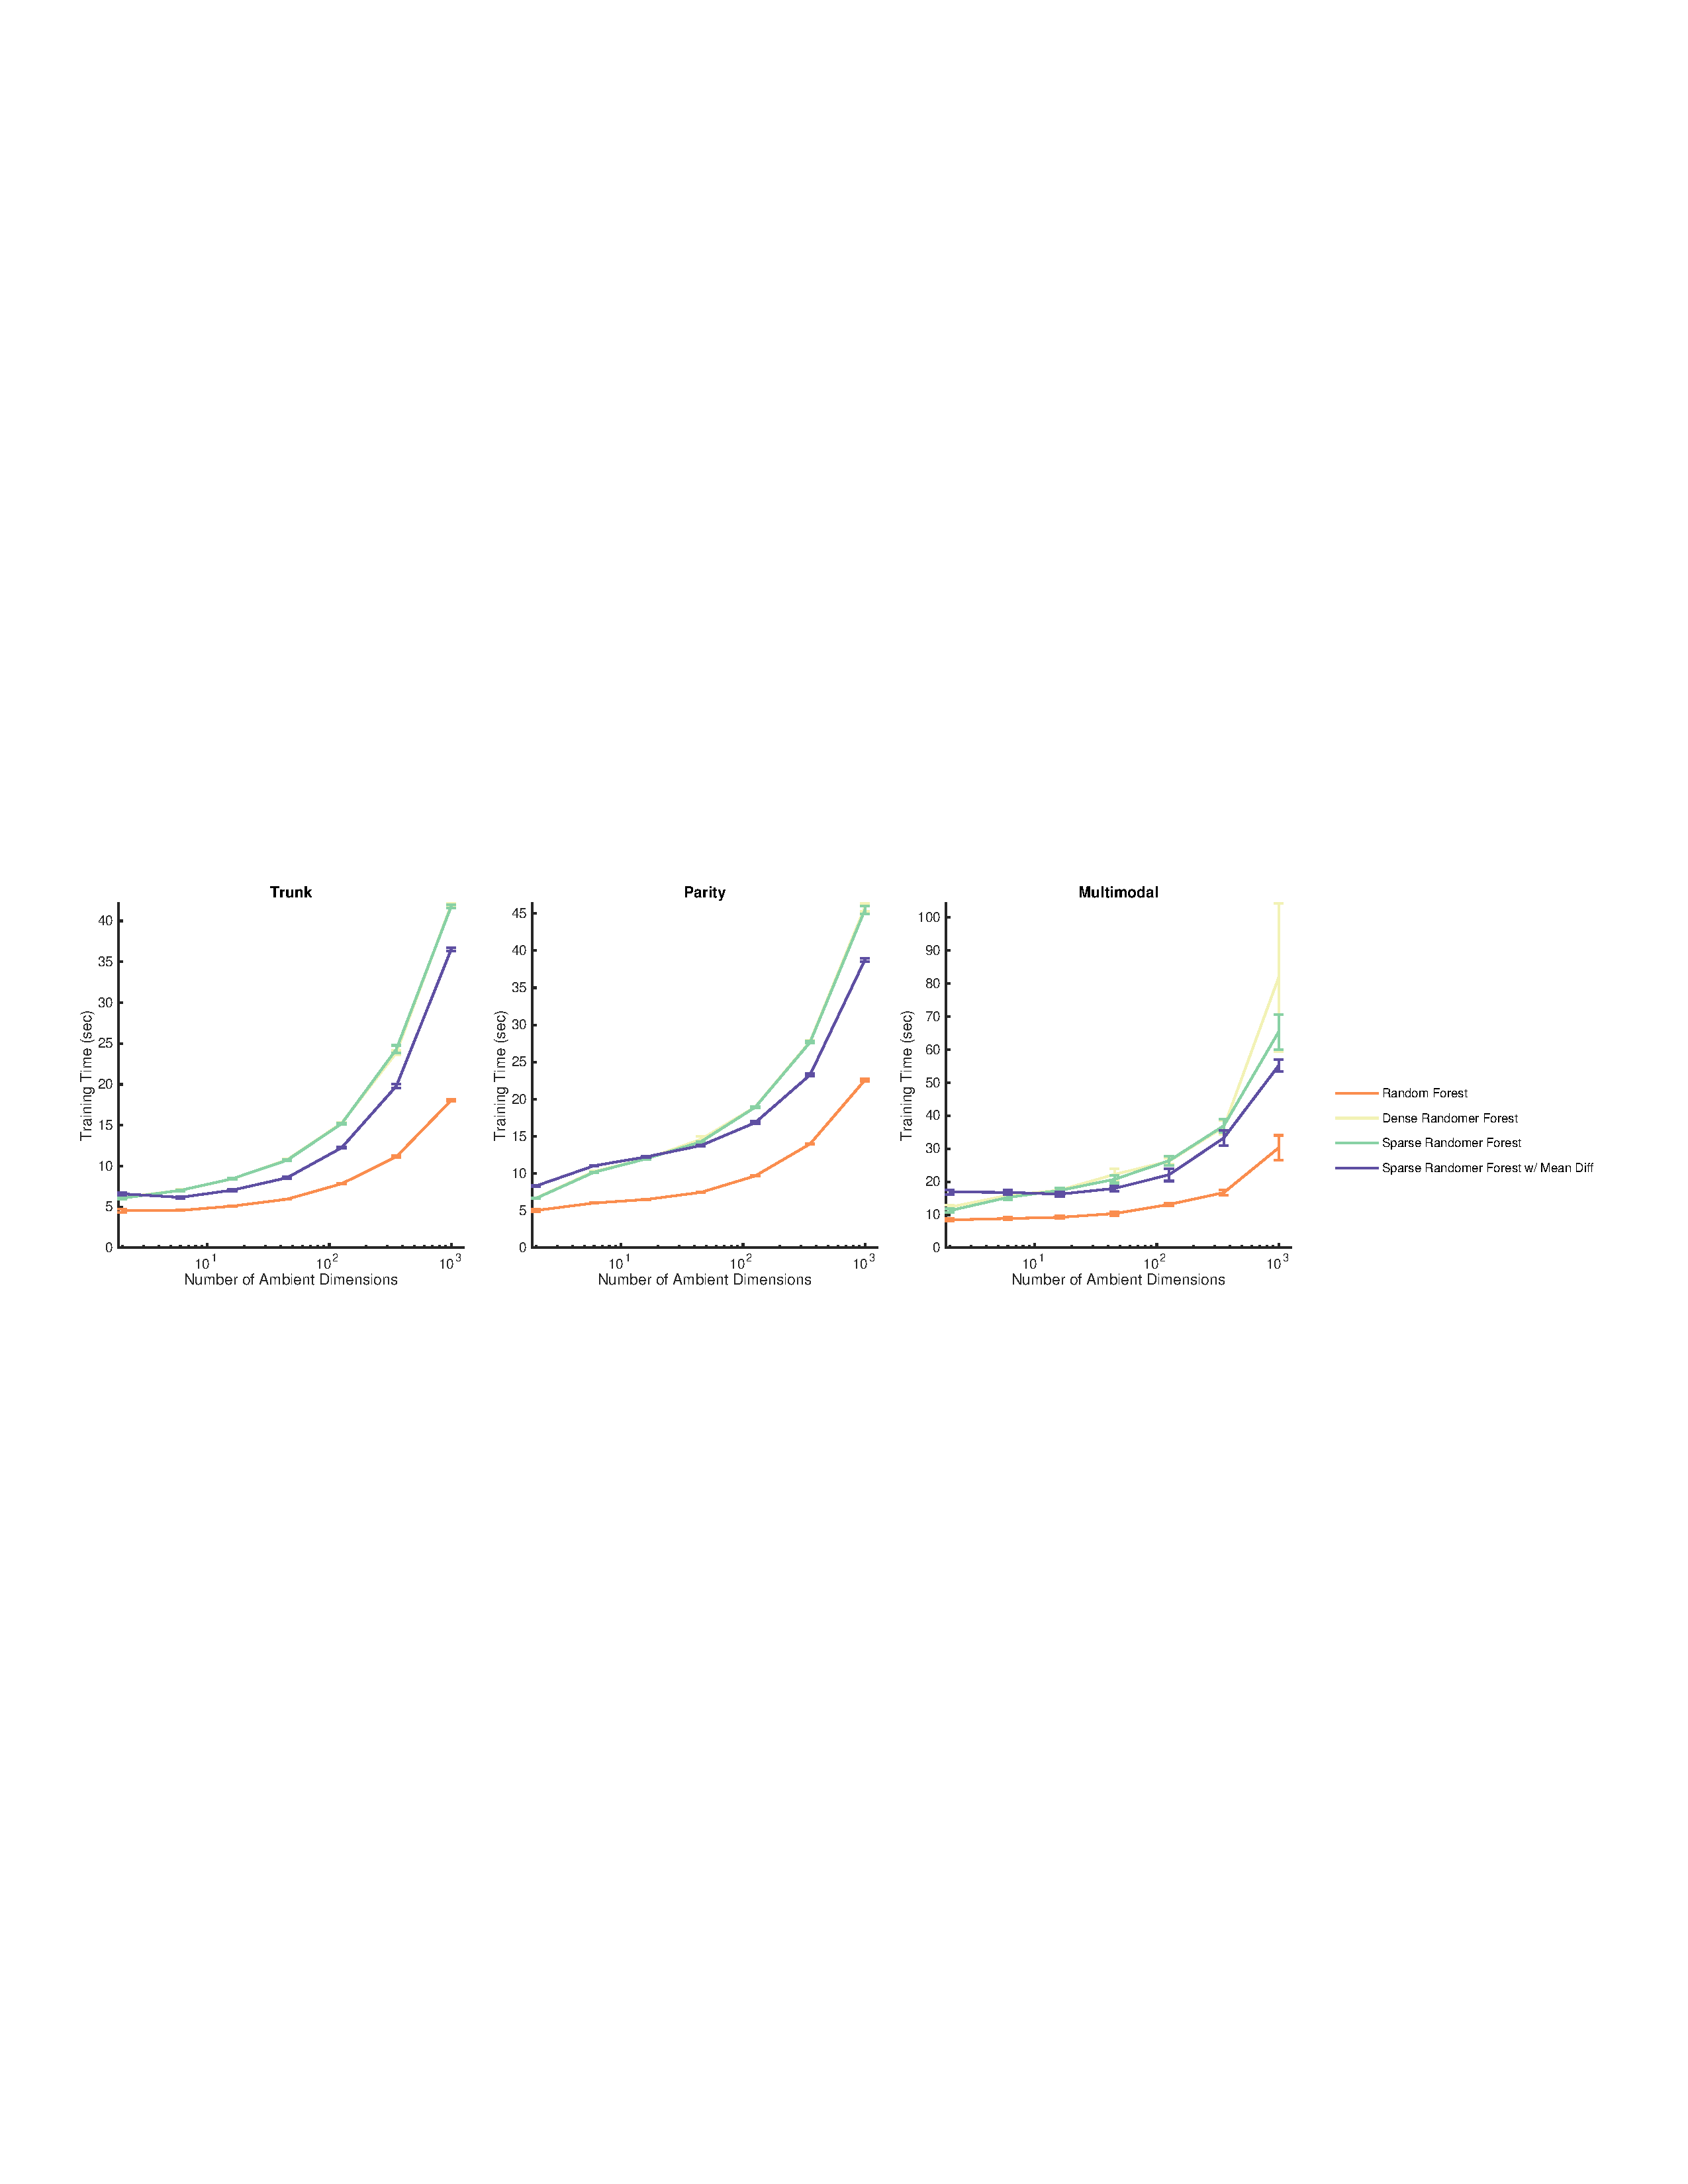
\includegraphics[trim=0in 3in 0in 3in, clip=true, width=\linewidth]{Fig2_Time}
\end{center}
\caption{Classifier training time comparing RF to several variants of RerF, same setting as the top row of Figure 1. The only difference is that the y-axis here labels training time (in seconds). Although RerF requires slightly more time than RF (largely due to random sampling of projection matrices), they scale similarly.}
\end{figure}

\begin{figure}[h]
\begin{center}
%\framebox[4.0in]{$\;$}
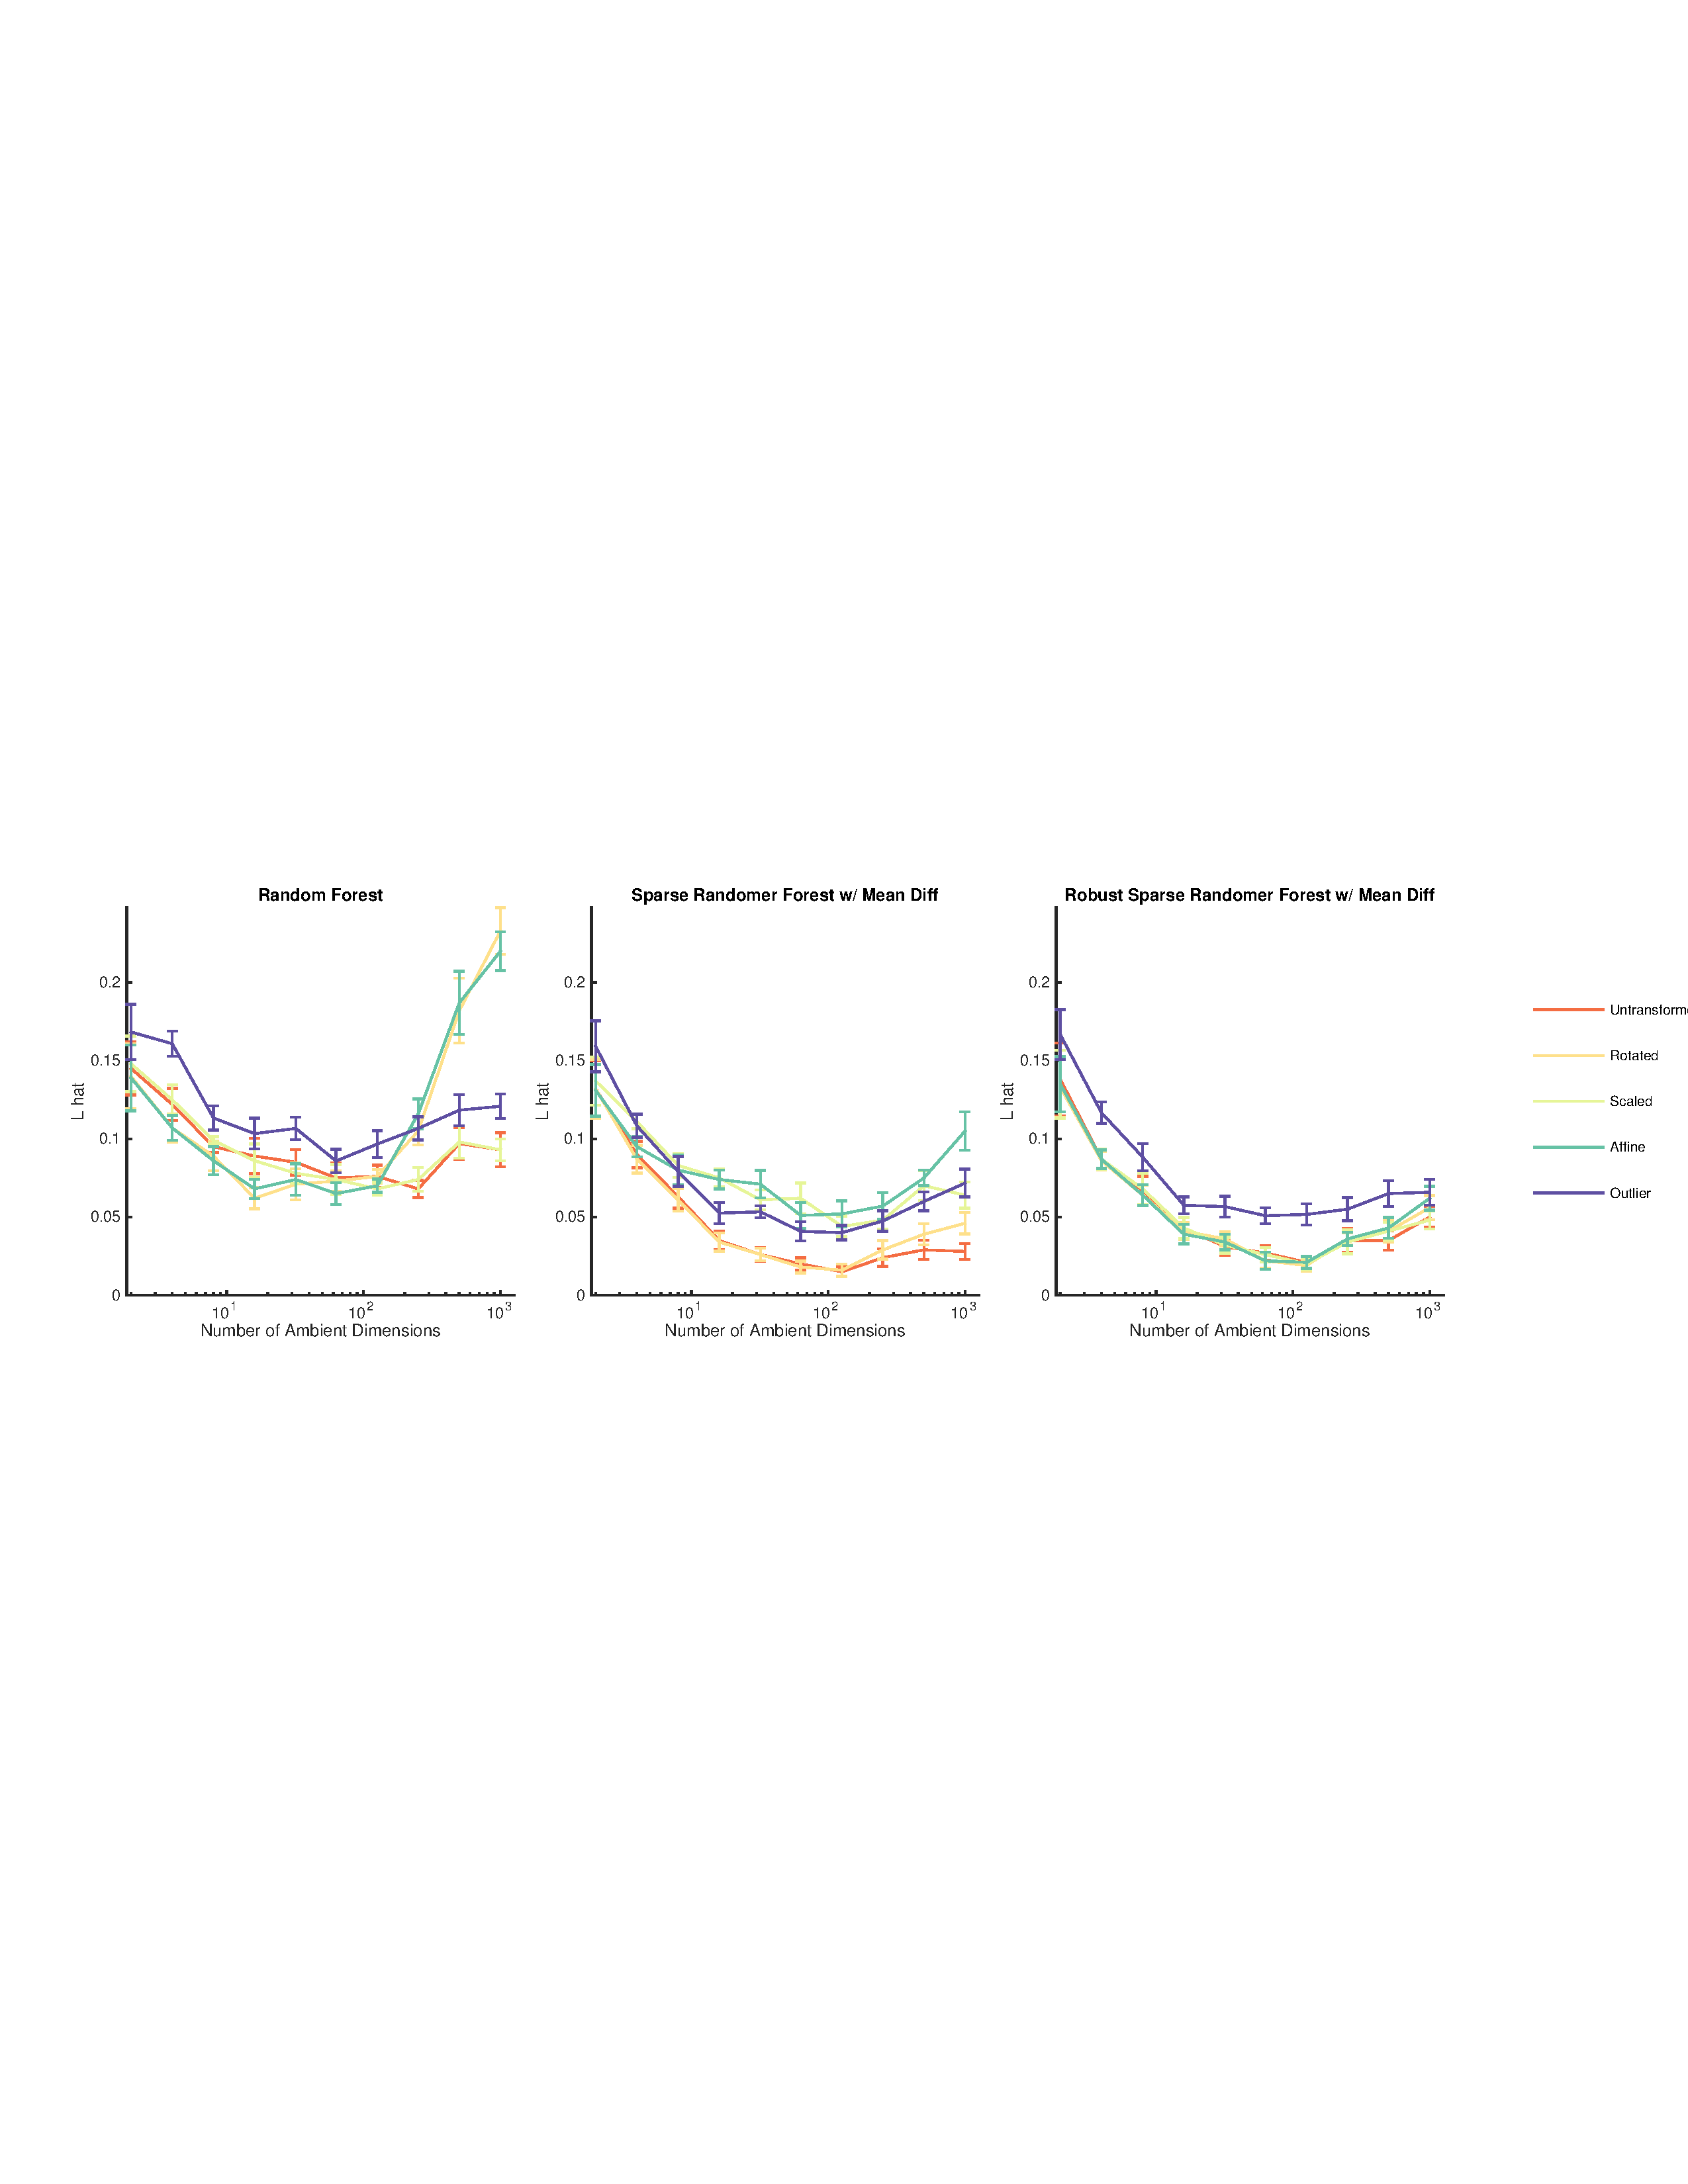
\includegraphics[trim=0in 0.9in 0in .09in, clip=true, width=\linewidth]{Fig3_Invariance_v2}
\end{center}
\caption{The effect of various transformations applied to the Trunk (panels A-D) and Parity (panels E-H) simulations (see Methods for details) on classification performance of (A,E) RF, (B,F) RerF (s+d), (C,G) RerF (s+d+r), and (D,H) Fisherfaces. Specifically, we consider, rotations, scalings, and affine transformations, as well as introducing outliers. Classification performance of RF is compromised by rotations and therefore affine transformations as well. RerF(s+d) is invariant to rotation, but not scaling and therefore not affine transformation. RerF(s+d+r) is invariant to to affine transformations. Like RerF (s+d), Fisherfaces is invariant to rotation but not scaling. Note that all variants are reasonably robust to outliers.}
\end{figure}

\begin{figure}[h]
\begin{center}
%\framebox[4.0in]{$\;$}
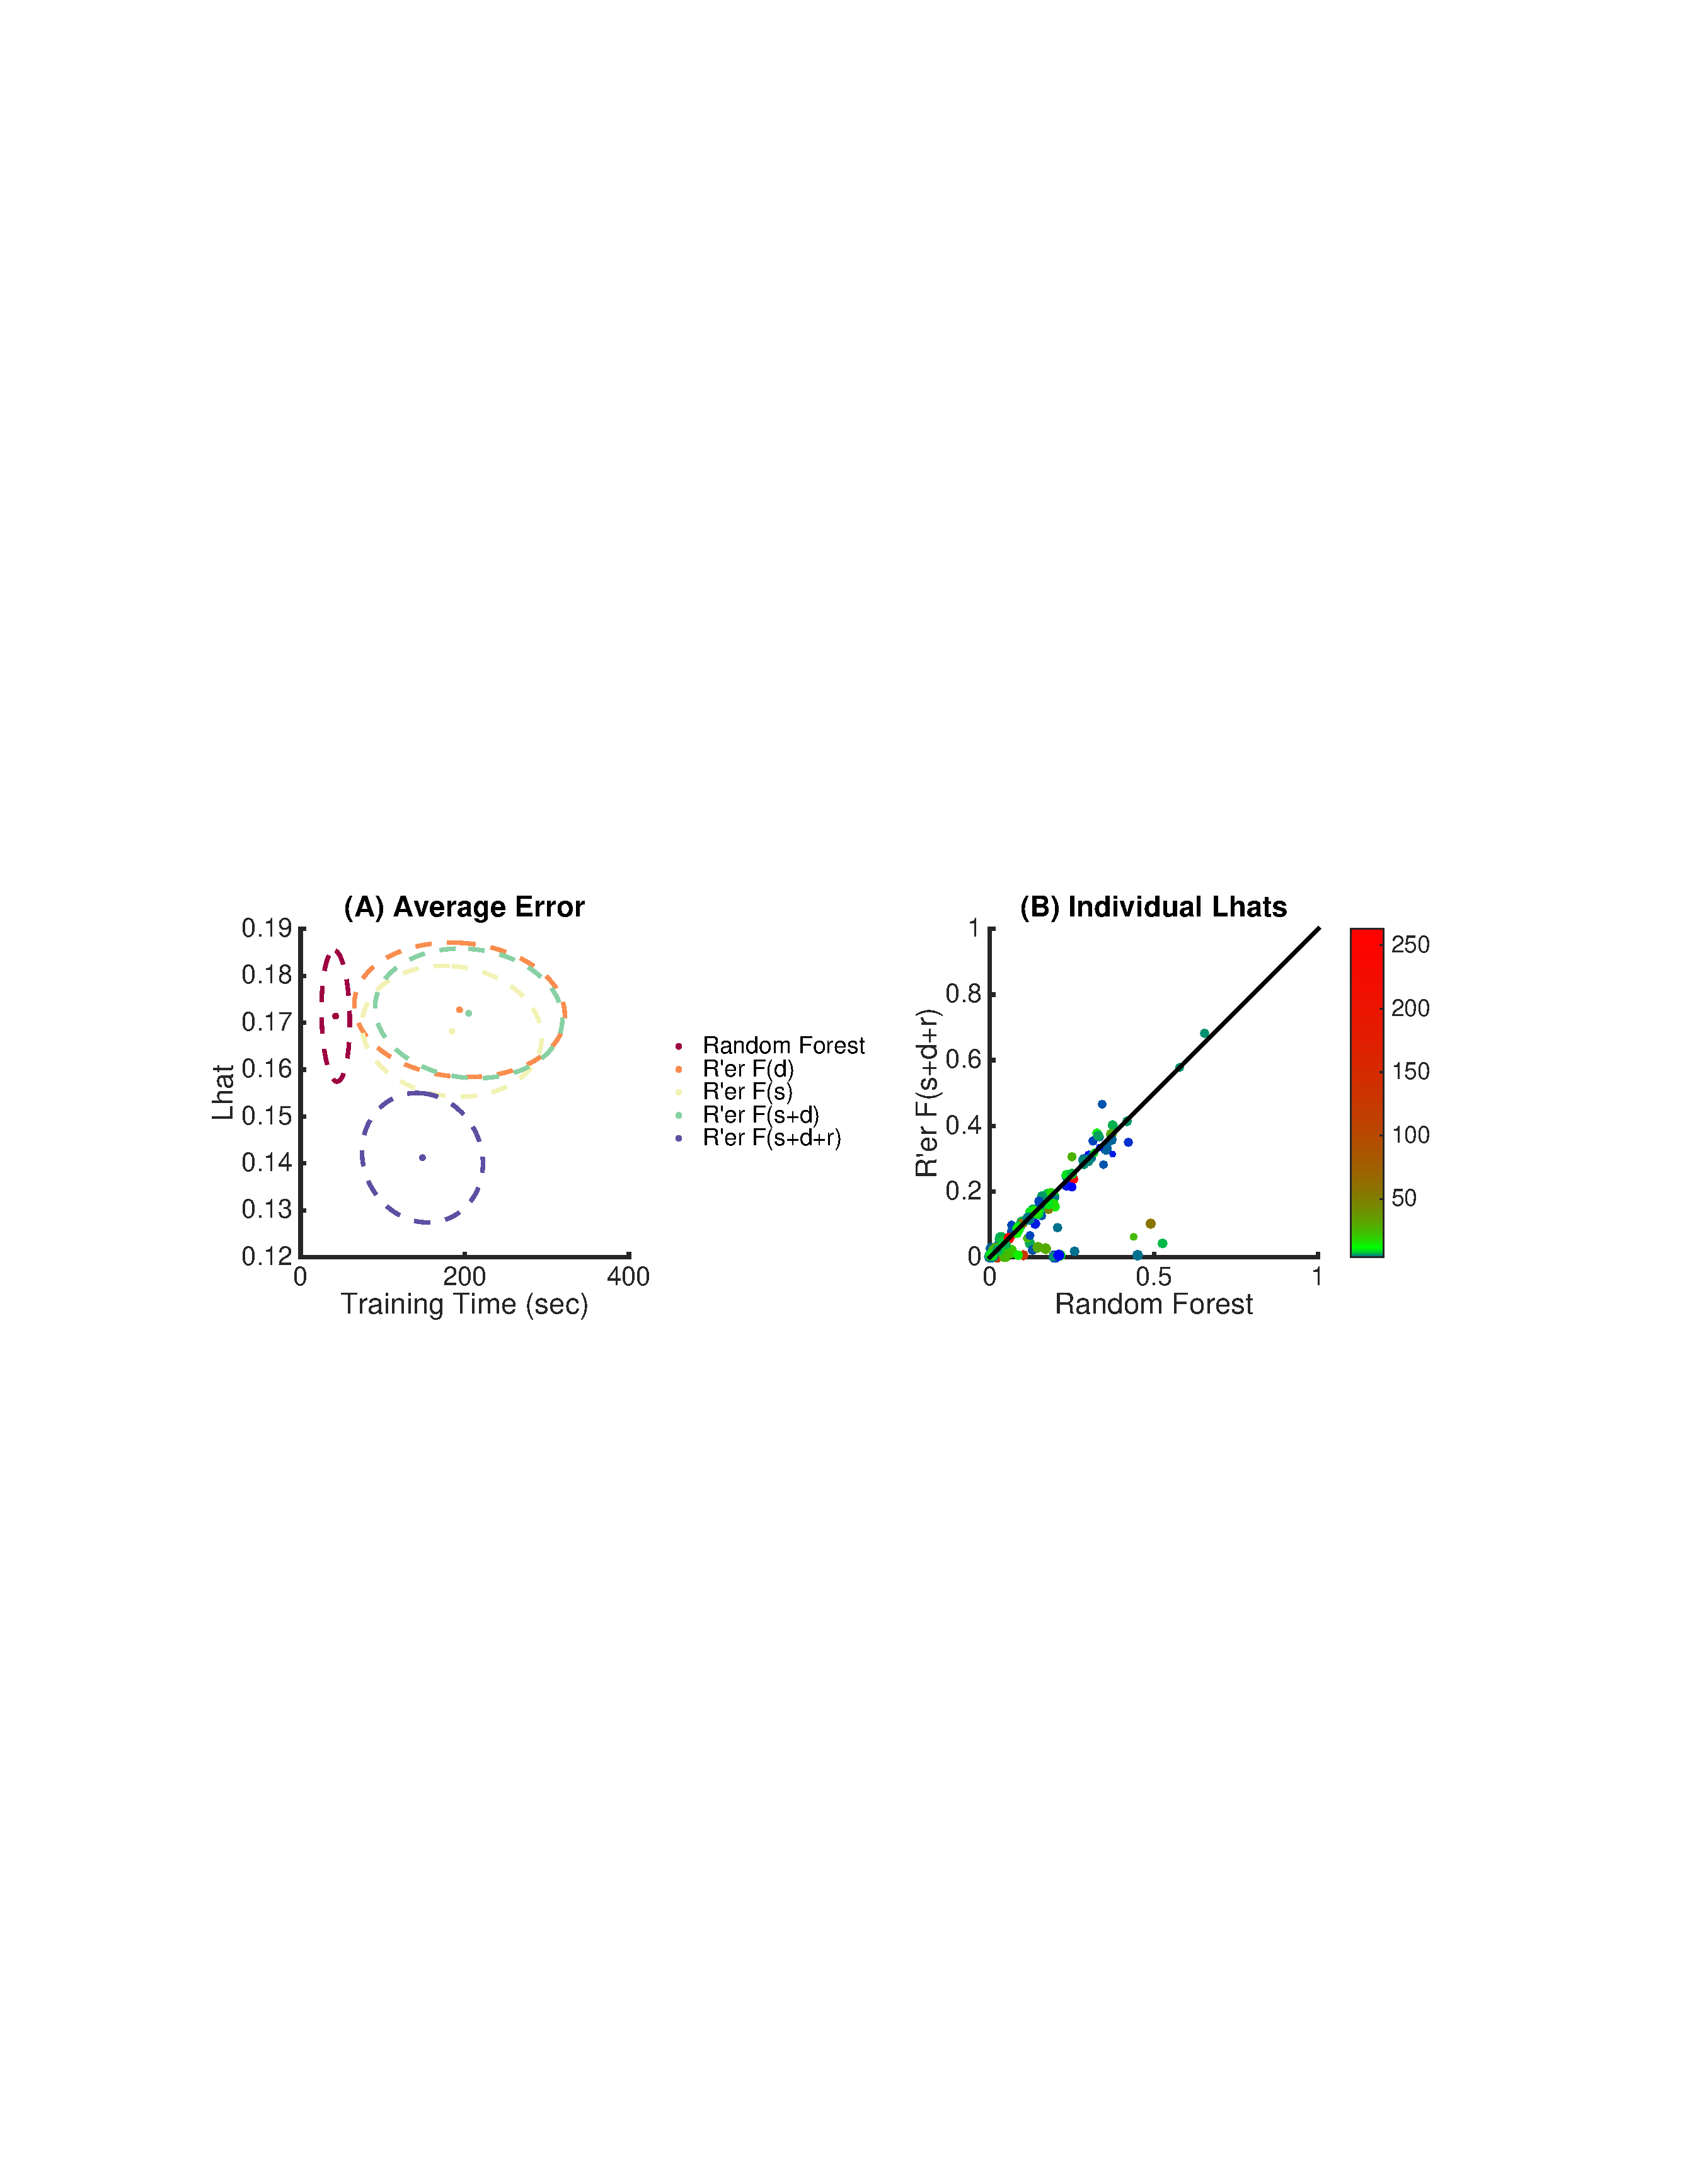
\includegraphics[trim=0in 2.3in 0in 2.3in, clip=true, width=\linewidth]{Fig4}
\end{center}
\caption{(A) Classification error and training time of Random Forest and Randomer Forests variants for all 121 datasets from the XXX benchmark comparison paper \cite{???}. (A) Average (dots) and 0.1 standard deviation level sets (dashed lines) for each method. (B) Classification error of Randomer Forest (sparse+delta+robust) vs. that of Random Forest for each of the 121 datasets. The black line indicates equal classification error of the two algorithms. Color indicates dimensionality of the datasets and size of points indicates number of samples. Note that RerF almost always does as well, and often significantly better.}
\end{figure}

\appendix
\setcounter{figure}{0}
\renewcommand\thefigure{A\arabic{figure}}
\begin{figure}[h]
\begin{center}
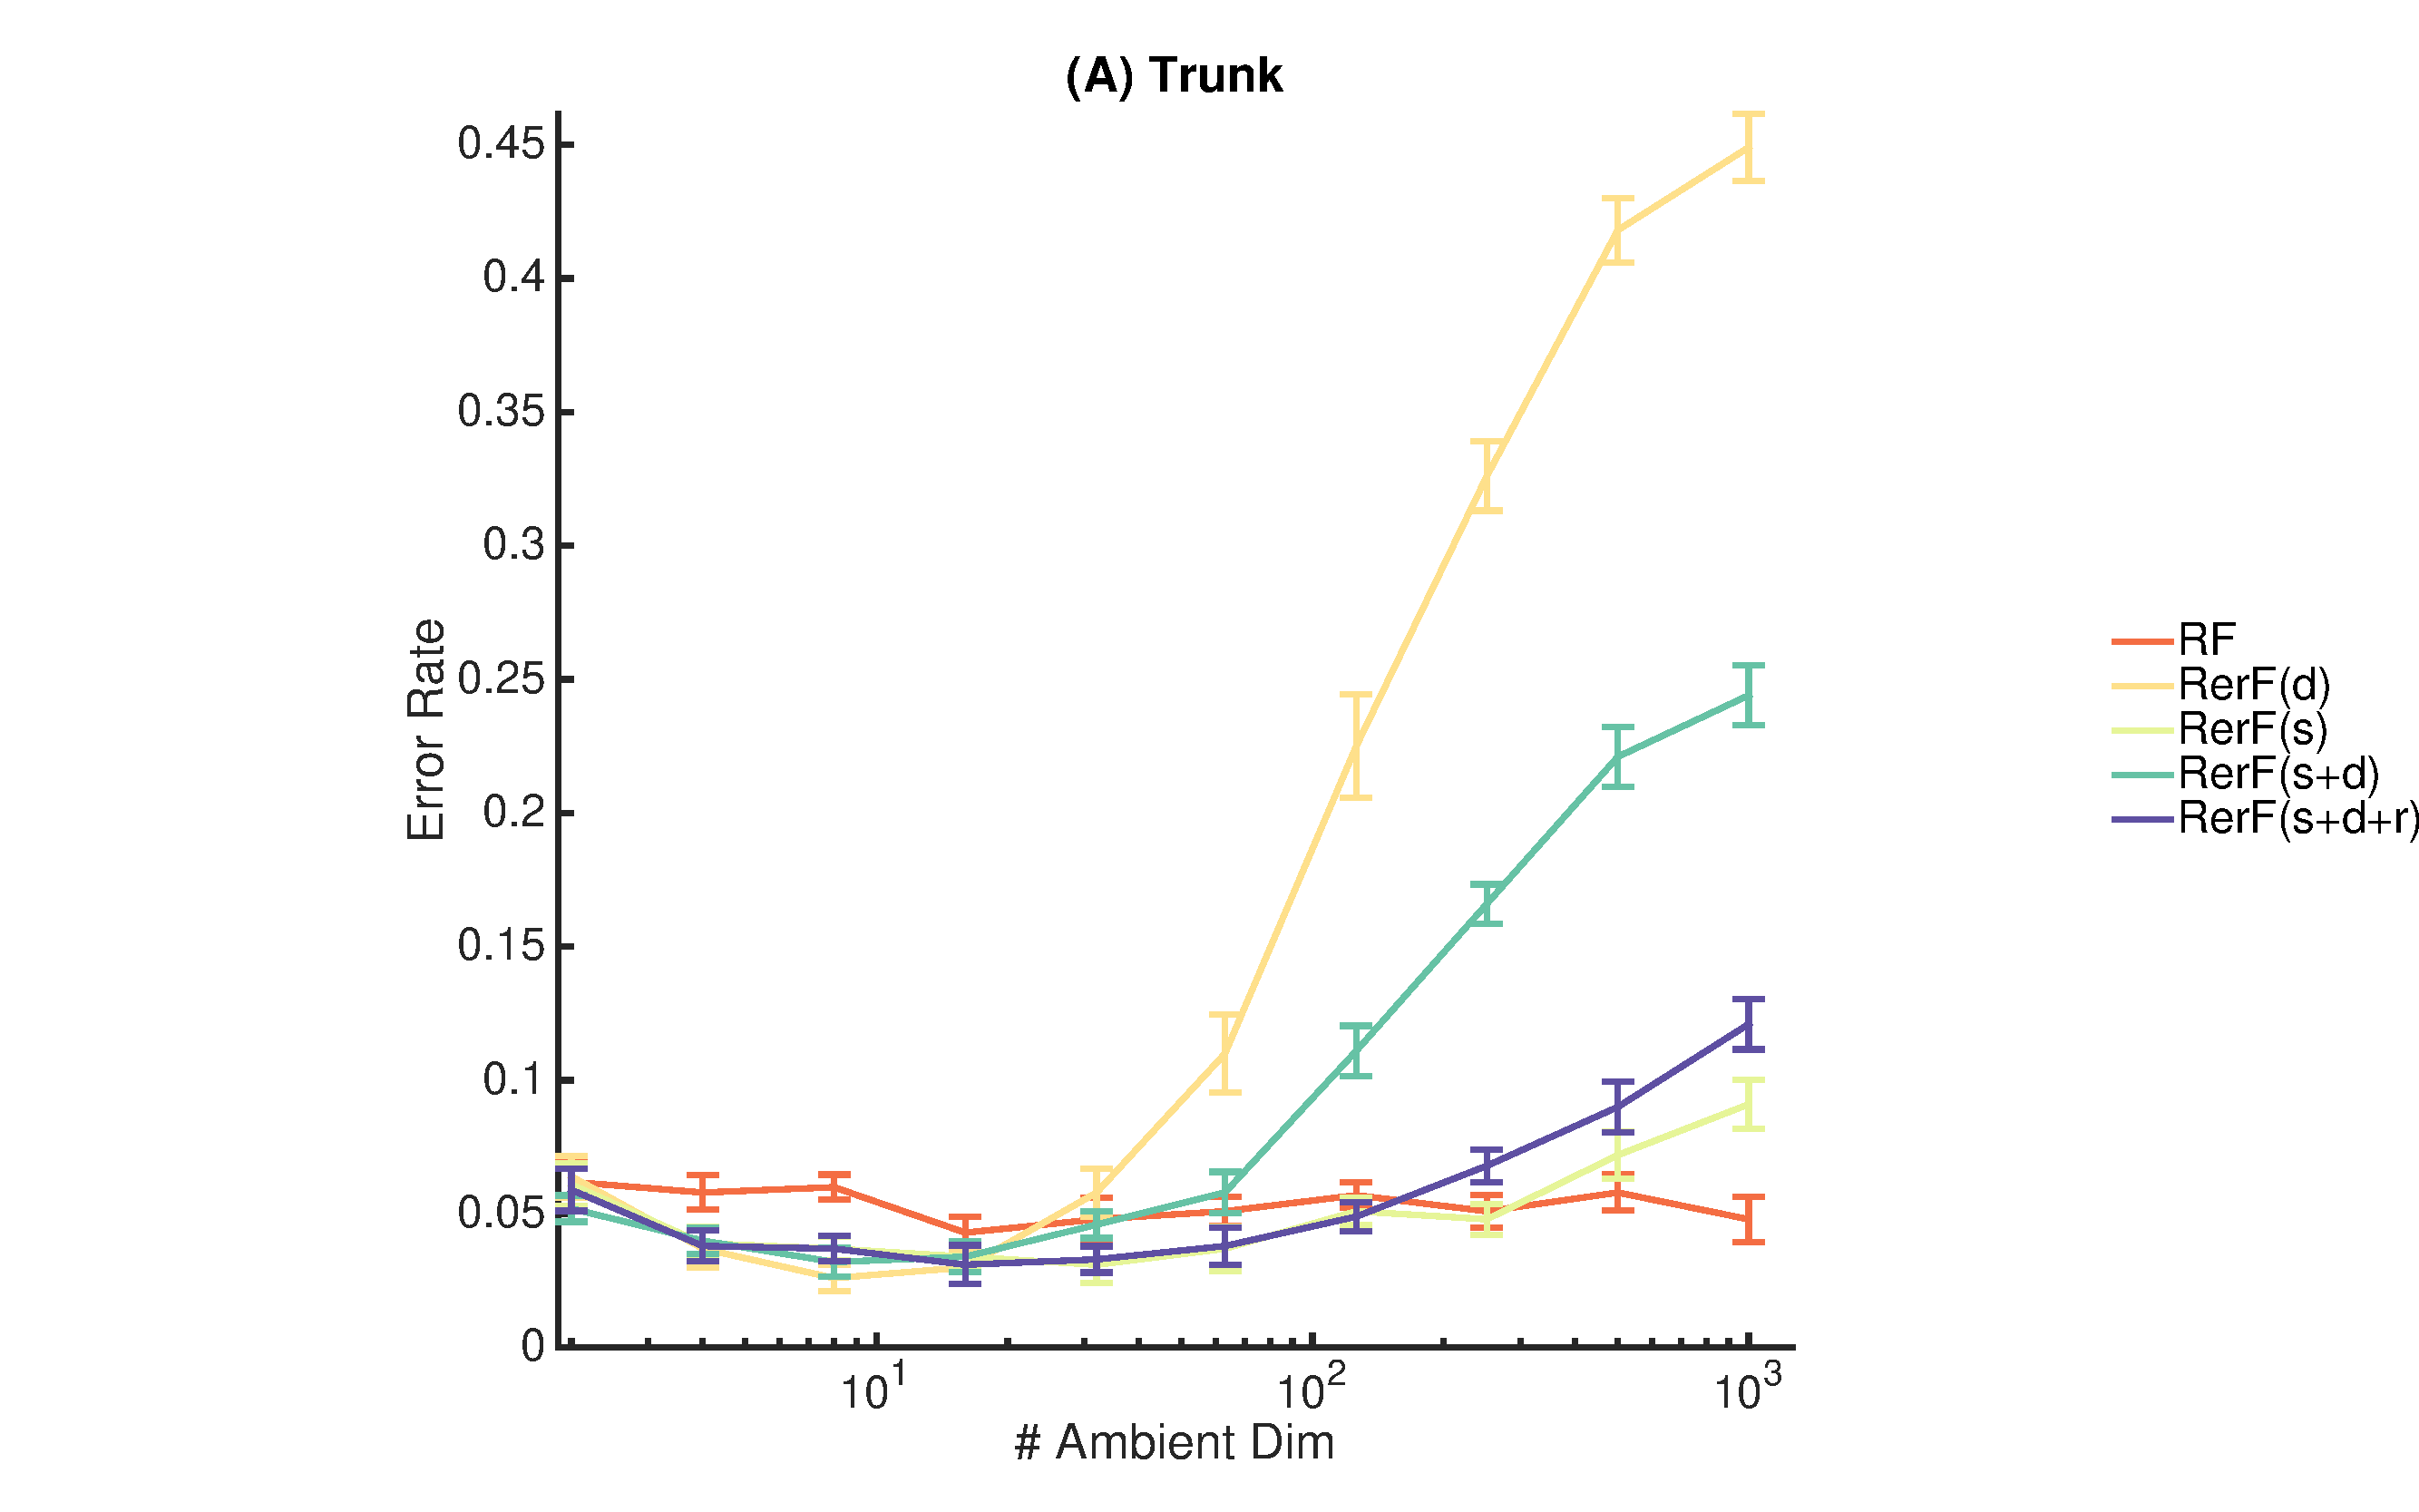
\includegraphics[trim=0in 0in 0in 0in, clip=true, width=\linewidth]{Trunk_hard}
\end{center}
\caption{Classification performance comparing Random Forest (RF) to several variants of Randomer Forest (RerF) on the modified Trunk simulation setting. Here, the ith diagonal of the covariance matrices of both classes is equal to the inverse of the difference in means of the ith dimension between the two classes. For small values of p, all variants of RerF perform marginally better than RF. For large values of p, all variants of RerF perform worse than RF.}
\end{figure}

\end{document}